\section{Theorie}
\label{sec:Theorie}

Ein Lock-In-Verstärker kann aus einem verrauschten Signal das rauschen herausfiltern und somit
das eigentliche Signal deutlicher machen. Ein verrauschtes Signal $U_{sig}$ läuft durch einen Bandpassfilter, wo es
von höheren und niedrigeren Frequenzen befreit wird. Danach wird es mit einem Referenzsignal $\omega_0$
multipiziert. Die Phasenlage $\phi$ des Referenzsignals kann mit einen Phasenschieber mit dem
verrauschtem Signal synchronisiert werden ($\Delta \phi = 0$). Ein darauffolgender Tiefpass integriert das Mischsignal
über mehrere Perioden der Modulationsfrequenz, wobei sich nicht zur Modulationsfrequenz synchronisierte Rauschbeiträge herausmitteln.
Die Ausgangsspannung ist dann proporional zur Eingangsapnnung und ist maximal bei einer Phasenverschiebung von $\phi = 0$.

\begin{equation}
  U_{out} \propto U_0 \cdot cos{\phi}
\end{equation}


Abbildung 1 zeigt den Aufbau eines Lock-In-Verstärkers.

\begin{figure}[H]
  \centering
  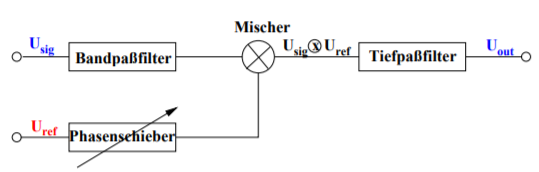
\includegraphics[height=5cm]{Lock.PNG}
  \caption{Allgemeiner Aufbau eines Lock-In-Verstärkers}
  \label{fig:Lock}
\end{figure}
